\documentclass{article}
\usepackage[a4paper, top=3cm, bottom=2.5cm, left=2.5cm, right=2.5cm]{geometry} % Ajuste de márgenes
\usepackage[spanish]{babel}
\usepackage[utf8]{inputenc}
\usepackage{tikz}
\usepackage{titling}
\usepackage{graphicx}
\usepackage{fancyhdr}
\usepackage{amsmath}
\usepackage{amssymb}
\usepackage{multicol}
\usepackage{cancel}
\usepackage{pgfplots}
\usepackage{hyperref}
\pgfplotsset{compat=1.18}
\usepackage{titlesec} % Para personalizar títulos
\usepackage{tocloft}  % Para mejorar el índice
\usepackage{setspace} % Para controlar el espaciado

% Configuración de Fancyhdr para encabezados y pies de página
\pagestyle{fancy}
\fancyhf{}
\fancyhead[L]{
\includegraphics[width=2cm]{assets/logo-utp.png}}
\fancyhead[R]{\textbf{Estadística descriptiva y probabilidades}}

\fancyfoot[R]{\thepage} % Número de página alineado a la derecha

% Ajustes de espaciado entre párrafos y márgenes superiores
\setlength{\parskip}{1.5em}
\setlength{\parindent}{0pt}
\setlength{\headheight}{17.26935pt} % Altura del encabezado
\addtolength{\topmargin}{-2.26935pt} % Compensar el aumento de la altura del encabezado
\setlength{\textheight}{23cm}  % Ajusta el alto del texto

% Definición de comandos personalizados
\newcommand{\SubItem}[1]{
    {\setlength\itemindent{15pt} \item[-] #1}
}

% Título del documento con mejor control de espaciado
\title{
  
\includegraphics[width=5cm]{./assets/logo-utp.png} \\
  \vspace{1cm}
  \textbf{Universidad Tecnológica del Perú} \\
  \vspace{2cm}
  \textbf{Análisis estadístico-descriptivo de la precipitación en el Perú durante el fenómeno de El Niño: diciembre 2023 a abril 2024} \\
  \vspace{1cm}
  \large \textbf{Para el curso de Estadística descriptiva y probabilidades.}
}
\author{
  \textbf{Luis Huatay Salcedo.} \\
  \texttt{hsluis4326@gmail.com} \\
  \texttt{U24218809 - 24229}
}


\begin{document}
\maketitle

\begin{center}
  Docente. Mg. Luis Fernando Velarde Vela  
\end{center}
\restoregeometry

\newpage

\begin{center}
  \textbf{\Large Índice}
\end{center}
\vspace{0.5cm} % Espacio entre título y contenido

\begin{spacing}{1.15} % Espaciado personalizado para mayor legibilidad
  \noindent
  \begin{enumerate}
    \item Introducción
    \item Problemática
    \item Objetivo general
    \begin{enumerate}
      \item Objetivos específicos
    \end{enumerate}
    \item Términos estadísticos
    \item Recolección de información
  \end{enumerate}
\end{spacing}

\newpage
\vspace*{\fill}
\section{Introducción}
El fenómeno de El Niño es un evento climático que ocurre en la región del Pacífico Sur, caracterizado por un calentamiento anómalo de las aguas del océano Pacífico, lo que provoca alteraciones en la circulación atmosférica y en la temperatura de la superficie del mar. En el Perú, este fenómeno se presenta de manera irregular en el tiempo y su duración suele abarcar los meses de diciembre a abril, cuando sus efectos se hacen evidentes tanto en la atmósfera, como en el terreno y el océano. Aunque El Niño es un fenómeno natural, en los últimos años se ha observado un aumento en su frecuencia e intensidad, lo que ha generado preocupación en la comunidad científica y en la población en general.

Este fenómeno trae consigo una serie de consecuencias desfavorables para el Perú, como lluvias intensas, inundaciones y deslizamientos de tierra. Sin embargo, también presenta aspectos favorables, como la recarga de acuíferos y la mejora en la agricultura. A pesar de estos beneficios, las consecuencias negativas son las que más preocupan a las autoridades y a la población, debido a su potencial para causar pérdidas humanas y materiales significativas.

En este contexto, el presente proyecto tiene como objetivo realizar un análisis estadístico-descriptivo de la precipitación en el Perú durante el fenómeno de El Niño, utilizando los conceptos, técnicas y herramientas aprendidas en el curso de Estadística Descriptiva y Probabilidades. Este análisis permitirá identificar patrones, tendencias y comportamientos que ayudarán a comprender mejor el fenómeno y a describir con mayor precisión su impacto en la precipitación.
\vspace*{\fill}

\newpage

\section{Problemática}

El fenómeno de El Niño es un evento climático que afecta a gran parte del planeta, y claramente, el Perú no es la excepción. Durante su ocurrencia se observan cambios significativos en la precipitación los cuales pueden tener consecuencias graves para la población y la economía del país, problemas como inundaciones, deslizamientos y pérdidas agrícolas son evidentes consecuencias que demandan soluciones de mitigación así como un enfoque de prevención. Dada la importancia de este fenómeno, resulta esencial comprender cómo varía la precipitación durante los trimestres más críticos, que en este caso son diciembre-enero-febrero (DEF), enero-febrero-marzo (EFM) y febrero-marzo-abril (FMA).

Sin un adecuado entendimiento estadístico de los patrones de precipitación trimestral durante El Niño, los esfuerzos de mitigación pueden ser insuficientes o ineficaces, lo que incrementa el riesgo de pérdidas humanas, económicas y ecológicas. Además, la imprevisibilidad del fenómeno puede llevar a malas decisiones en la gestión de recursos hídricos y la planificación de infraestructura, aumentando la vulnerabilidad de las comunidades expuestas. Por lo tanto, la falta de análisis detallado de la precipitación limita la capacidad de anticiparse a los riesgos, dejando al país menos preparado para enfrentar este fenómeno recurrente.

\begin{figure}[h]
  \centering
  \begin{minipage}{0.45\textwidth}
      \centering
      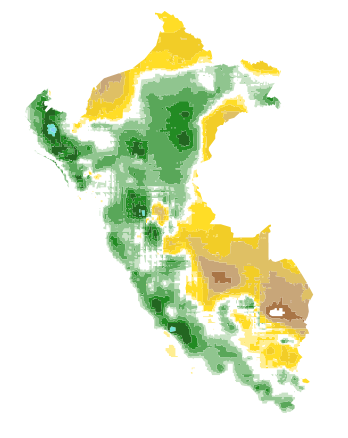
\includegraphics[width=\textwidth]{./assets/2016_Diciembre.png}
      \caption{Promedio precipitación DEF 2017.}
  \end{minipage}
  \hfill
  \begin{minipage}{0.45\textwidth}
      \centering
      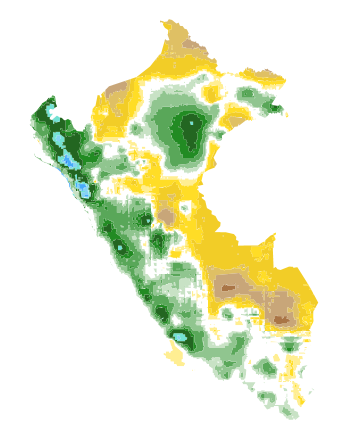
\includegraphics[width=\textwidth]{./assets/2017_abril.png}
      \caption{Promedio de precipitación FMA 2017.}
  \end{minipage}
  \label{fig:1}
\end{figure}
  Comparación entre los trimestres DEF y FMA en 2017. Se puede observar como la precipitación en el trimestre FMA es mayor que en DEF especialmente en las zona de la costa Sur.

\newpage

\section{Objetivo general}

Realizar un análisis estadístico-descriptivo de la precipitación en el Perú durante el fenómeno de El Niño en el periodo comprendido entre diciembre del 2016 y abril del 2017, con el fin de identificar patrones, tendencias y comportamientos que permitan comprender mejor el impacto del fenómeno en la precipitación.

\subsection{Objetivos específicos}

\begin{enumerate}
  \item \textbf{Identificar y caracterizar} las variables climáticas en los datos obtenidos de precipitación trimestral durante los periodos DEF, EFM y FMA, y definir el tipo de muestreo empleado para la recolección de los datos relacionados con el fenómeno de El Niño en el Perú.
  
  \item \textbf{Organizar los datos} de precipitación en una tabla de frecuencias, categorizándolos por rangos de valores y periodos trimestrales, y presentar visualmente esta información mediante gráficos que faciliten la comparación entre los trimestres estudiados.
  
  \item \textbf{Calcular y comparar} las medidas de tendencia central (media, mediana y moda) de la precipitación para cada trimestre, describiendo las diferencias entre los periodos y analizando los patrones emergentes en las regiones más afectadas por el fenómeno.
  
  \item \textbf{Evaluar la variabilidad} de los datos de precipitación mediante el cálculo de las medidas de dispersión (varianza, desviación estándar y coeficiente de variación) para entender la magnitud de las fluctuaciones en la precipitación durante los trimestres analizados.
  
  \item \textbf{Identificar y describir} las medidas de posición (percentiles, cuartiles) y analizar la forma de la distribución de la precipitación (asimetría y curtosis) para obtener una visión más profunda de los comportamientos extremos y atípicos durante los meses afectados por el fenómeno de El Niño.
  
  \item \textbf{Más}
\end{enumerate}

\newpage

\section{Términos estadísticos}

A continuación, se presentan los términos estadísticos que se utilizarán en el análisis de los datos de precipitación en el Perú durante el fenómeno de El Niño. La mayor parte de las definiciones están tomadas de Gaviria y Márquez (2019), con ajustes específicos al contexto del estudio.

\begin{enumerate}
  \item \textbf{Población:} Una población $P$ se entiende como un conjunto de elementos u objetos de interés sobre el cual se realizan las observaciones. Dado que los objetos o cosas cuentan con una cantidad finita o infinita de proyecciones, se entiende una población como una característica asociada a los objetos que pertenecen a $P$.
  
  Para este caso la población estará conformada por los datos de precipitación en el Perú recopilados de manera intermitente según fuente desde 1982.

  \item \textbf{Muestra:} Por otro lado, dada una poblanción $P$, una muestra $M$ es un subconjunto representativo de la población $P$.
  
  La muestra se selcciona a fin de obtener una representación adecuada de la población, en este caso, se tomarán los datos de precipitación de los trimestres DEF, EFM y FMA de fines del año 2023 y comienzos del 2024.

  \item \textbf{Unidad de análisis:} La unidad de análisis es el objeto o cosa que se observa en una investigación estadística. En este caso, la unidad de análisis será la precipitación en milímetros en las diferentes regiones del Perú durante los trimestres DEF, EFM y FMA.
  
  \item \textbf{Variable:} Es una característica que puede ser medida o categorizada en una población o muestra. Las variables pueden ser cualitativas o cuantitativas.
  
  Para nuestra unidad de análisis se considerará la variable cuantitativa de tipo discreta de la precipitación en milímetros.

  \item \textbf{Paŕametro:} Es un valor numérico $\theta$ que resume una población P. Un parámetro es una característica de la población.
  
  En este caso los parámetros son deducibles a partir del análisis visual de la información gráfica y tabular de los datos de precitpitación de los años en general.

  \item \textbf{Estadístico:} Es un valor numérico que resume a la muestra. Por otro lado, es también una función de los datos muestrales.
  
  En este caso, los estadísticos serán las medidas de tendencia central, dispersión y posición que se calcularán a partir de los datos de precipitación en los trimestres DEF, EFM y FMA.
\end{enumerate}

\newpage

\section{Recolección de información}

La recolección de información se realizará a partir de datos históricos de precipitación en el Perú durante el fenómeno de El Niño, recopilados de la fuente oficial y de autoría, \textbf{Dirección de Meteorología y Evaluación Ambiental Atmosférica SENAMHI} Los datos se obtendrán de las estaciones meteorológicas ubicadas en diferentes regiones del país, que registran la precipitación en milímetros durante los trimestres DEF, EFM y FMA.

Así mismo estos datos se encuentran en los repositorios espaciales del \textbf{IDESEP} (La infraestructura de Datos Espaciales del SENAMHI PERU) que son un conjunto de políticas, estándares, procesos, tecnologías y recursos humanos que se encuentran integrados y destinados a facilitar la producción, estandarización, uso y acceso a la información geoespacial del SENAMHI, teniendo como base la información estandarizada, oficial y oportuna para la toma de decisiones.

Puede acceder al repositorio oficial desde este enlace:

\texttt{https://idesep.senamhi.gob.pe/geoserver/web/}

Algunos datos sobre el desarrollo y autoría tomados de la fuente de metadatos oficiales de la información:

\begin{itemize}
  \item \textbf{Autor:} Sub Dirección de Predicción Climática (SPC)
  \item \textbf{Punto de contacto:} Patricia Porras Vásquez (Especialista en Servicios Climáticos de Los Trópicos)
  \item \textbf{Email:} pporras@senamhi.gob.pe
  \item \textbf{Identificador:} d6e9a47a-2b78-4f8e-ad07-2c3e6f8f7b9e
  \item \textbf{Fecha de publicación:} Jueves 26 de septiembre del 2024
\end{itemize}

\begin{figure}[ht]
  \centering
  \begin{minipage}{0.45\textwidth}
      \centering
      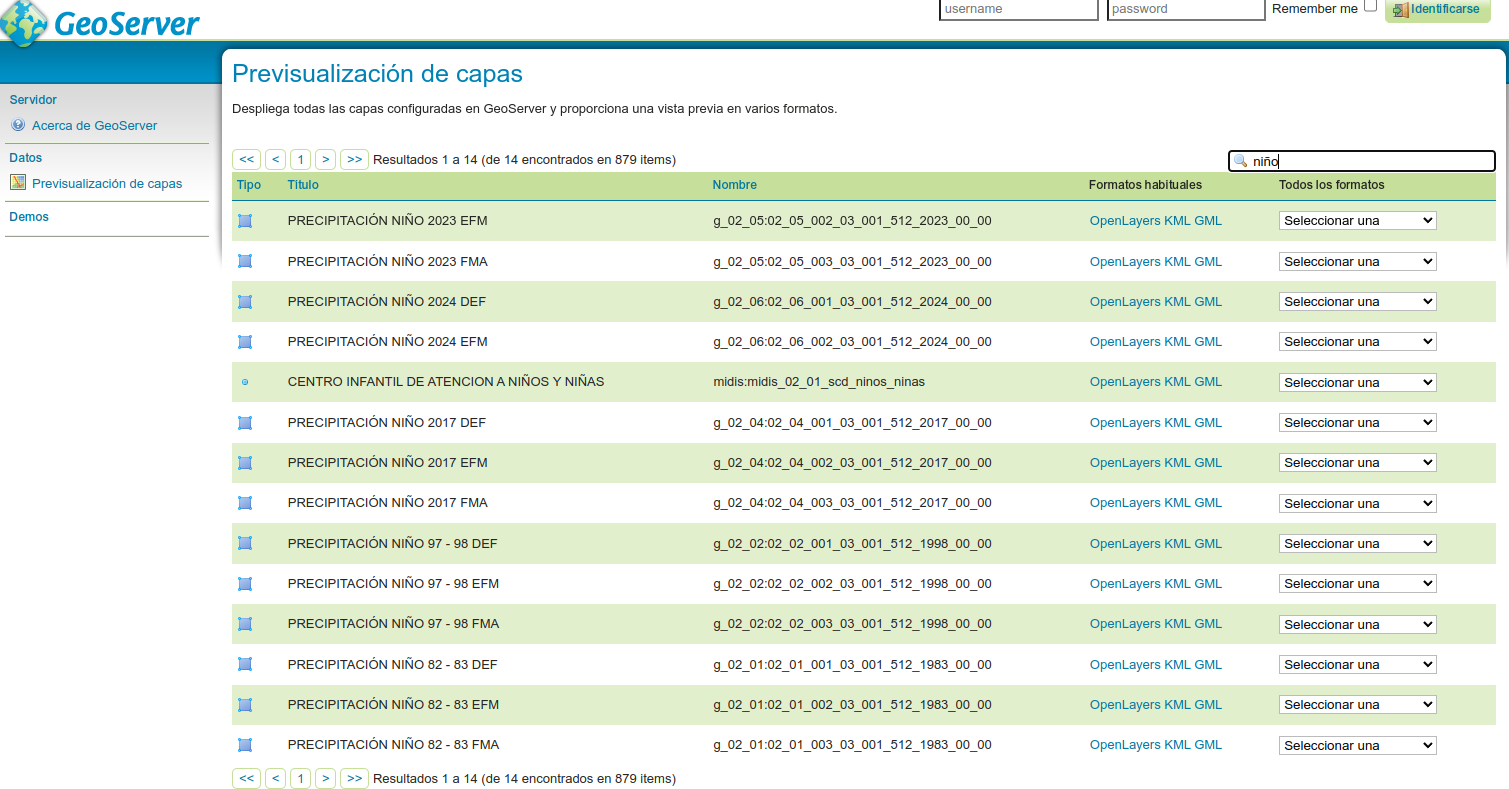
\includegraphics[width=\textwidth]{./assets/Geoserver_IDESEP.png}
      \caption{Repositorio oficial \textbf{IDESEP}.}
  \end{minipage}
  \hfill
  \begin{minipage}{0.45\textwidth}
      \centering
      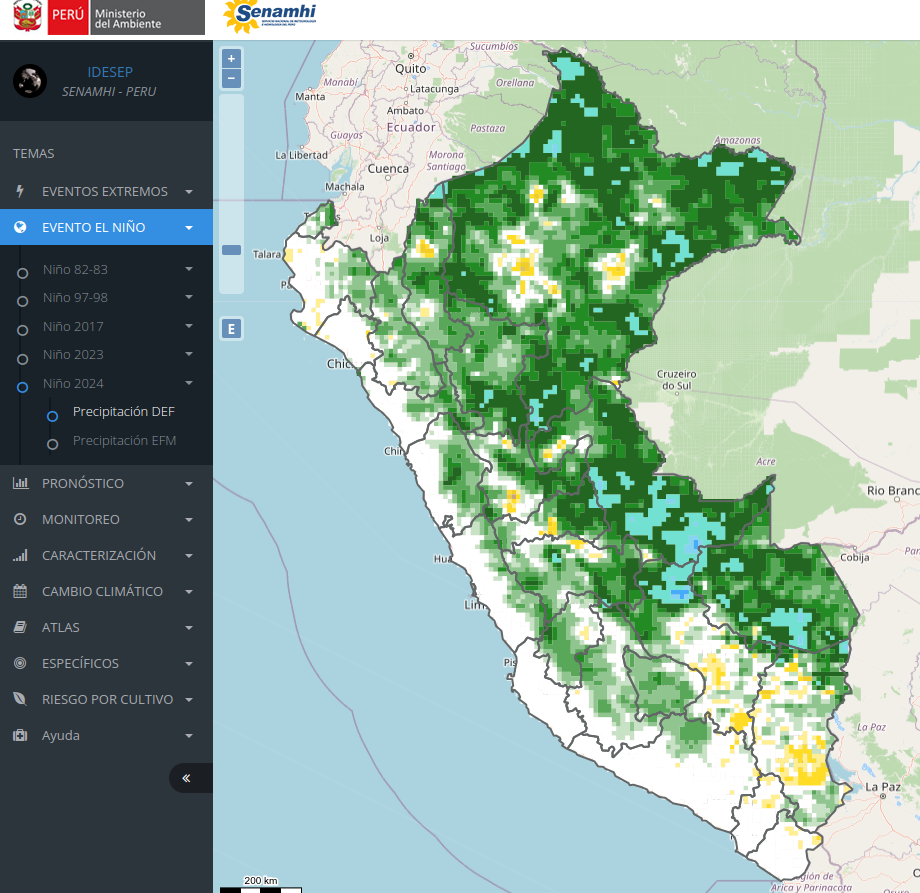
\includegraphics[width=\textwidth]{./assets/Geovisor.png}
      \caption{Geovisor \textbf{SENAMHI}.}
  \end{minipage}
  \label{fig:2}
\end{figure}

\newpage

\begin{thebibliography}{9}

  \bibitem{IDESEP} 
  IDESep - Infraestructura de Datos Espaciales del SENAMHI. (n.d.). SENAMHI. Repositorio de datos geoespaciales hidrológicos. Recuperado de \url{https://idesep.senamhi.gob.pe/geoserver/web/}
  
  \bibitem{Metadatos} 
  Metadatos de la Información IDESep. (n.d.). SENAMHI. Recuperado de \href{https://idesep.senamhi.gob.pe/geonetwork/srv/spa/catalog.search#/metadata/d6e9a47a-2b78-4f8e-ad07-2c3e6f8f7b9e}{IDESEP - Geonetwork}

  \bibitem{Estadística} 
  Gaviria Peña, C., \& Márquez Fernández, C. A. (2019). \textit{Estadística descriptiva y probabilidad}. Editorial Bonaventuriano. 

\end{thebibliography}
  
\end{document}